\documentclass[tikz,border=15pt]{standalone}
\usepackage{amsmath,amssymb}
\usetikzlibrary{arrows.meta, shadows}
\usepackage[T1]{fontenc}
\usepackage[utf8]{inputenc}
\usepackage{newpxtext,newpxmath}
\usepackage{sectsty}
%% Define colors to match the requested style's naming convention
%\definecolor{accent}{RGB}{20, 80, 180}       % A deep structural blue
%\definecolor{softgray}{RGB}{244, 246, 248}   % Light background gray for ambient space
%\definecolor{softaccent}{RGB}{220, 230, 250} % Soft blue for the subspace plane
\definecolor{accent}{HTML}{1F4E79}
\definecolor{softaccent}{HTML}{EAF2F8}
\definecolor{softgray}{HTML}{F6F7F9}
% Custom macros
\newcommand{\F}{\mathbb{F}}
\newcommand{\code}{\mathcal{C}}
\newcommand{\vect}[1]{\mathbf{#1}}

\begin{document}
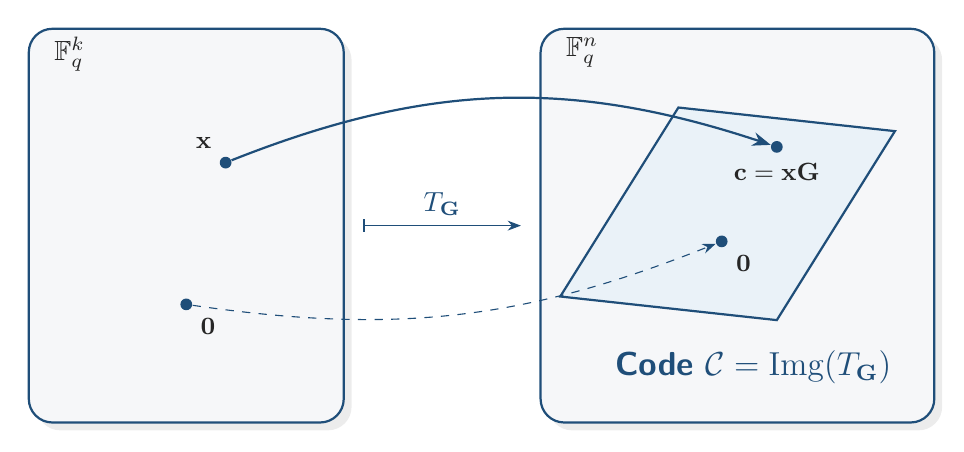
\begin{tikzpicture}[
	>=Stealth,
	ambient/.style={
		draw=accent, thick, fill=softgray, rounded corners=3mm, 
		minimum width=5cm, minimum height=5cm,
		drop shadow={opacity=0.15, shadow xshift=1mm, shadow yshift=-1mm}
	},
	labeltext/.style={text=black!85},
	header/.style={font=\bfseries\sffamily\large, text=accent},
	codeword/.style={circle, fill=accent, inner sep=1.5pt}
	]
	
	% ==========================================
	% PANEL 1: Message Space F_q^k
	% ==========================================
	
	% Ambient Space (Message Space)
	% Overriding minimum width slightly to reflect k < n
	\node[ambient, minimum width=4cm] (space1) at (0,0) {};
	\node[anchor=north west, labeltext] at (space1.north west) {\; $\F_q^k$};
	
	% The origin of the message space
	\node[codeword, label={[labeltext, font=\small]below right:$\vect{0}$}] (zero_k) at (0,-1) {};
	
	% A unique message vector x
	\node[codeword, label={[labeltext, font=\small]above left:$\vect{x}$}] (x) at (0.5, 0.8) {};
	
	% ==========================================
	% PANEL 2: Ambient Space F_q^n & Code Subspace C
	% ==========================================
	
	% Ambient Space
	\node[ambient] (space2) at (7,0) {};
	\node[anchor=north west, labeltext] at (space2.north west) {\; $\F_q^n$};
	
	% Code Subspace (im(T_G))
	% Using a plane to visually represent that it is a k-dimensional subspace
	\draw[draw=accent, thick, fill=softaccent] 
	(4.75, -.9) -- (6.25, 1.5) -- (9.0, 1.2) -- (7.5, -1.2) -- cycle;
	\node[header] at (7.2, -1.8) {Code $\code = \operatorname{Img}(T_\mathbf{G})$};
	
	% The origin (Linear code must contain 0)
	\node[codeword, label={[labeltext, font=\small]below right:$\vect{0}$}] (zero_n) at (6.8,-0.2) {};
	
	% The resulting codeword c = xG
	\node[codeword, label={[labeltext, font=\small]below:$\mathbf{c} = \vect{x}\mathbf{G}$}] (c) at (7.5, 1.0) {};
	
	% ==========================================
	% LINEAR TRANSFORMATION (T_G) ARROWS
	% ==========================================
	
	% Mapping of the message vector to its unique codeword
	\draw[->, accent, thick] (x) to[bend left=20] 
	node[midway, above, labeltext, font=\small\sffamily] {} (c);
	
	% Mapping of the origin (showing linearity)
	\draw[->, accent, thin, dashed] (zero_k) to[bend right=15] (zero_n);
	
	\draw[|->, accent, thin] (2.25,0) -- (4.25,0) node[midway, above] {$T_{\mathbf{G}}$};
\end{tikzpicture}
\end{document}